% Created 2017-10-16 Mon 11:24
% Intended LaTeX compiler: pdflatex
\documentclass[11pt]{article}
\usepackage[utf8]{inputenc}
\usepackage{lmodern}
\usepackage[T1]{fontenc}
\usepackage{fixltx2e}
\usepackage{graphicx}
\usepackage{longtable}
\usepackage{float}
\usepackage{wrapfig}
\usepackage{rotating}
\usepackage[normalem]{ulem}
\usepackage{amsmath}
\usepackage{textcomp}
\usepackage{marvosym}
\usepackage{wasysym}
\usepackage{amssymb}
\usepackage{amsmath}
\usepackage[version=3]{mhchem}
\usepackage[numbers,super,sort&compress]{natbib}
\usepackage{natmove}
\usepackage{url}
\usepackage{minted}
\usepackage{underscore}
\usepackage[linktocpage,pdfstartview=FitH,colorlinks,
linkcolor=blue,anchorcolor=blue,
citecolor=blue,filecolor=blue,menucolor=blue,urlcolor=blue]{hyperref}
\usepackage{attachfile}
\usepackage[left=1in, right=1in, top=1in, bottom=1in, nohead]{geometry}
\geometry{margin=1.0in}
\usepackage{hyperref}
\usepackage{amsmath}
\usepackage{graphicx}
\usepackage{epstopdf}
\usepackage{fancyhdr}
\pagestyle{fancy}
\fancyhf{}
\usepackage[labelfont=bf]{caption}
\usepackage{setspace}
\setlength{\headheight}{10.2pt}
\setlength{\headsep}{20pt}
\renewcommand{\headrulewidth}{0.5pt}
\renewcommand{\footrulewidth}{0.5pt}
\lfoot{\today}
\cfoot{\copyright\ 2017 W.\ F.\ Schneider}
\rfoot{\thepage}
\chead{\bf{Advanced Chemical Engineering Thermodynamics (CBE 60553)\vspace{12pt}}}
\lhead{\bf{Homework 6}}
\rhead{\bf{Due November 3, 2017}}
\usepackage{titlesec}
\titlespacing*{\section}
{0pt}{0.6\baselineskip}{0.2\baselineskip}
\title{University of Notre Dame\\Advanced Chemical Engineering Thermodynamics\\(CBE 60553)}
\author{Prof. William F.\ Schneider}
\usepackage{siunitx}
\usepackage[version=3]{mhchem}
\def\dbar{{\mathchar'26\mkern-12mu d}}
\setcounter{secnumdepth}{3}
\author{William F. Schneider}
\date{\today}
\title{CBE 60553 Homework}
\begin{document}

\begin{OPTIONS}
\end{OPTIONS}

\noindent \textbf{Solve each problem on separate sheets of paper, and clearly indicate the problem number and your name on each.  Carefully and neatly document your answers.  You may use a mathematical solver like Matlab or Mathematica. Use plotting software for all plots.}

\section{It all adds up now}
\label{sec:org5c913f6}
The diagram below describes the energy states available to some molecule.

\begin{figure}[htbp]
\centering
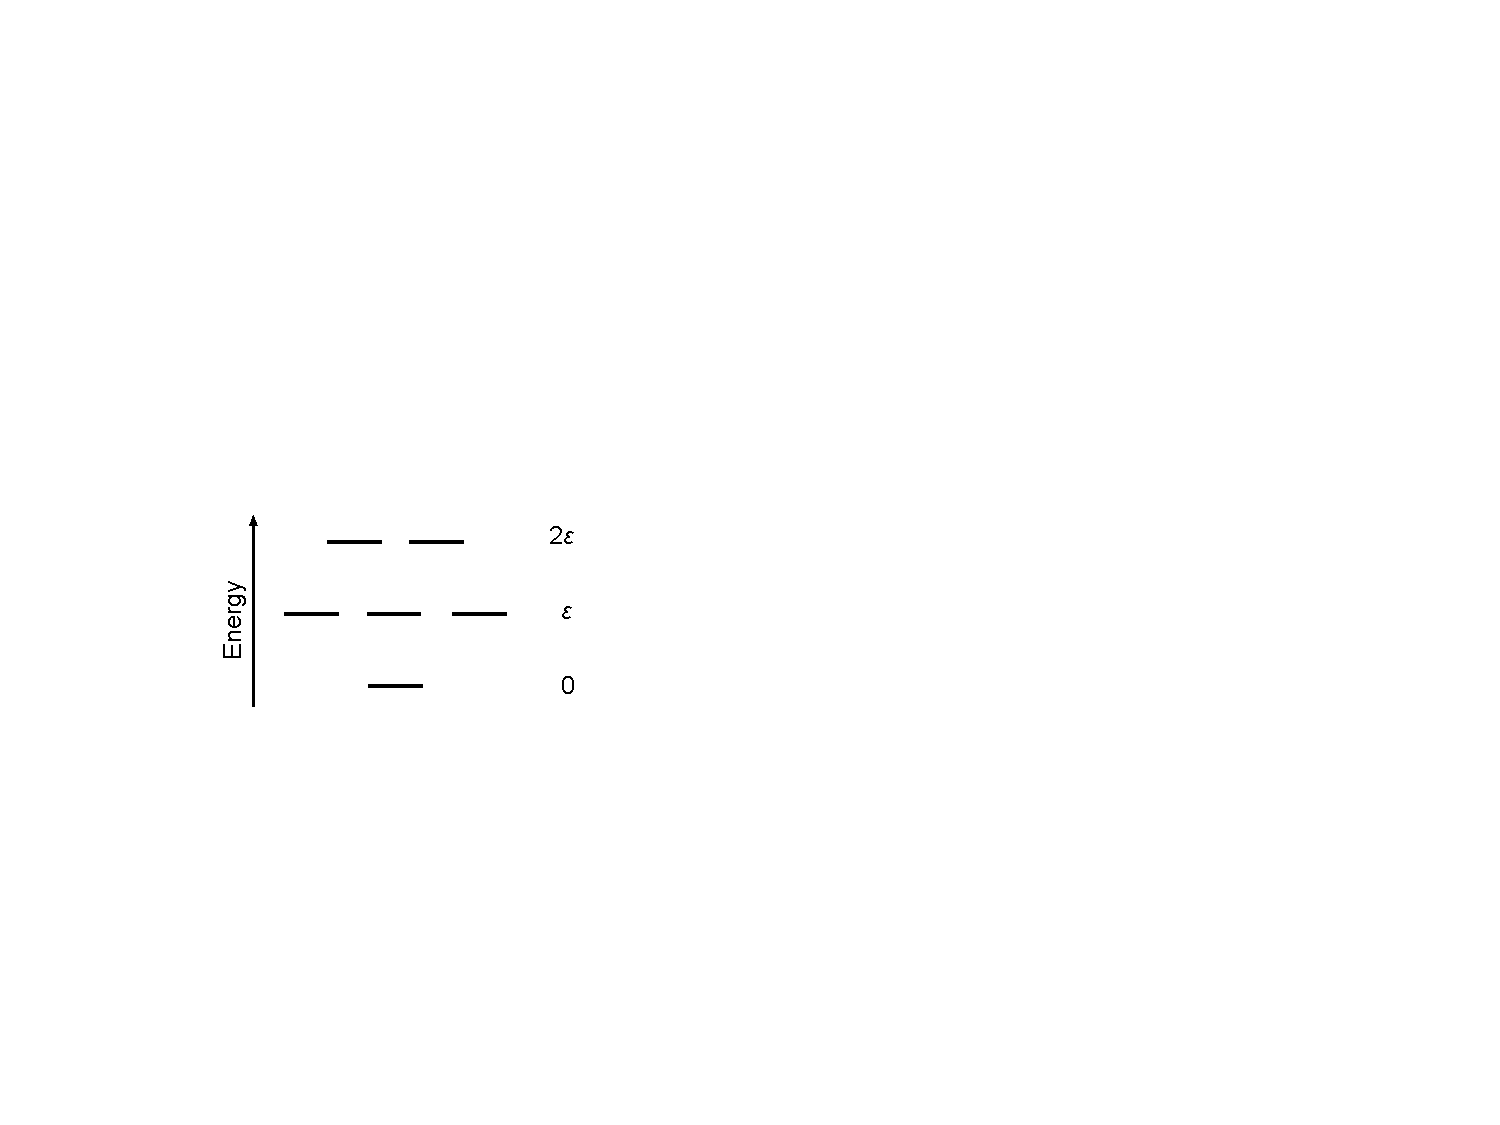
\includegraphics[width=3in]{./figs/Six-state.pdf}
\end{figure}

\begin{enumerate}
\item \label{q:Q} Construct the partition function \(q\) for the molecule at thermal equilibrium at a
temperature \(\beta = 1/k_b T\).
\item \label{q:prob} Plot the probability for the molecules to have each of the three possible energies
as a function of temperature.  Be sure to indicate the probabilities in the limits
\(T\rightarrow 0\) and \(T\rightarrow\infty\).
\item \label{q:U} Derive an expression for the energy \(u\) per molecule by summing over the possible
configurations weighted by their probabilities.  Plot this average energy vs.~
temperature.  Be sure to indicate the probabilities in the limits \(T\rightarrow 0\) and \(T\rightarrow\infty\).
\item Derive an expression for the energy \(u\) per molecule by taking the appropriate
derivative of the partition function from question \ref{q:Q}.  Does your result agree
with that from question \ref{q:U}?
\item Derive an expression for the Helmholtz free energy \(f\) per molecule from the
partition function.  Plot \(f\) vs.~temperature, assuming \(\epsilon/k_b=300~\text{K}\).
\item \label{q:S} Derive an expression for the entropy \(s\) per molecule from the
partition function.  Plot \(s\) vs.~temperature, again assuming \(\epsilon/k_b=300~\text{K}\).
\item Look at your answers for questions \ref{q:prob} and \ref{q:S}.  Can you use them
to rationalize the Third Low of thermodynamics?
\item What would happen to the Third Law if the ground (\(\epsilon = 0\)) state was degenerate?
\end{enumerate}

\section{Thermodynamics from scratch}
\label{sec:orgd4f0e7b}
Let's calculate the thermodynamic properties
of an ideal gas of \ce{CO2} at 1 bar pressure.  \ce{CO2} is a linear molecule (you knew
that, right?), has a rotational constant \(B=0.3836~\text{cm}^{-1}\) and vibrational
frequencies \(\mu_i = 2349\), 1388, 667, and 667\textasciitilde{}cm\(^{-1}\).

\begin{enumerate}
\item Calculate the translational, rotational, and four vibrational temperatures of \ce{CO2}.
\item Plot the total translational, rotational, and total vibrational \emph{energies} of
\ce{CO2} from \(T=\) \SIrange[range-units = single]{200}{2000}{K}.  Which (if any) of the three types of motions dominate
the internal energy?
\item Plot the total translational, rotational, and total vibrational \emph{Helmholtz energies} of
\ce{CO2} from \(T=\) \SIrange[range-units = single]{200}{2000}{K}.  Which (if any) of the three types of motions dominate
the Helmholtz energy?
\item Plot the total translational, rotational, and total vibrational \emph{constant
  volume molar heat capacities} of
\ce{CO2} from \(T=\) \SIrange[range-units = single]{200}{2000}{K}.  Which (if any) of the three types of motions dominate
the heat capacity?
\end{enumerate}
\section{How'd the scratching turn out?}
\label{sec:org6d33433}
Ideal gas thermodynamic quantities are often tabulated in polynomials of
  temperature.  The molar heat heat capacity of \ce{CO2} is reported by a source to be:
\begin{equation*}
  C_p^\text{ig}(t) = -11.401074 - 55.231532t+5.149108t^2-0.29158t^3+0.110128t^{-2}+115.93493t^{1/2}
\end{equation*}
\noindent where \(t=T(K)/1000\).  Compare (by plotting) this expression to your
\(C_v^\text{ig}(T)\) from scratch.  Recall \(C_p^\text{ig} = C_v^\text{ig}+R\).

\section{Langmuir isotherm}
\label{sec:org29ff83e}
Let's estimate an adsorption isotherm for CO on Pt at \SI{600}{K}, a temperature of practical relevance to catalysis:
\begin{equation}
  \ce{\text{*} + CO (g) <=> CO\text{*}}
\end{equation}
\noindent Suppose the CO gas is ideal, has a rotational constant
  \(B=\SI{1.931}{\per\centi\meter}\) and a harmonic \ce{C-O} stretch frequency of
  \SI{2150}{\per\centi\meter}.  CO binds C-end down, one CO/Pt, with a constant binding
  energy of about \SI{150}{\kilo\joule\per\mole}.  The surface-bound CO has (about) the
  same \ce{C-O} stretch frequency and rotational constants as in the gas. In addition, the
  CO vibrates againt the metal surface with a frequency of about
  \SI{500}{\per\centi\meter} and parallel to the surface with frequency
  \SI{150}{\per\centi\meter} (2-fold degenerate because the CO can move in two orthogonal
  directions parallel to the surface).

\begin{enumerate}
\item Estimate the adsorption equilibrium constant \(K(T)\) at \SI{600}{K}.  Use a gas standard
state of \SI{1}{bar}. Recall we derived in class that
\end{enumerate}
\[
 K(T) = \frac{q_\text{site}(T)}{q^{\circ}_\text{gas}(T)} e^{-\Delta{E}/k_{B}T}
\]

\begin{enumerate}
\item Plot the adsorption isotherm vs.~pressure.  At what pressure do you expect the surface to be 50\% covered with CO?
\end{enumerate}
\end{document}